
\subsection{Fair-Aware Re-ranking/Personalized Fair-Aware Re-ranking}

Microlending is the provision of small and low-interest loans (as little as \$25) to low-income individuals or small-scale entrepreneurs from under-developed countries  \cite{yunus1998banker}. The extremely poor people in rural areas often lack collateral, steady employment, or a verifiable credit history, hence they cannot get access to financial services. Under such circumstances, microlending has attracted an increased attention in the last decade \cite{chen2017microfinance}, providing impoverished entrepreneurs an opportunity to start their own businesses as well as avoid the vicious cycle of debt.

One of the leading international microlending organizations, Kiva Microfunds (Kiva.org), has crowd-funded about 3 million borrowers with \$1.27 billion USD as of February 2019 \cite{kiva}. Kiva does not collect interest but provides an intermediary service for lenders and borrowers, as illustrated in Figure \ref{fig:kiva_process}. Borrowers from over 80 countries, divided into 8 regions by Kiva, post their applications for loans on the website for lenders to support. Lenders browse and crowd-fund the loans in the increments of \$25 or more. 
%After 

% % recommender systems, personalization
Loan recommender systems \cite{choo2014gather,choo2014understanding} are designed to assist lenders in looking for promising borrowers. Such systems model lenders' historical behaviors and generate personalized recommendations to meet the lenders' interests or needs. While these recommender systems aim to provide efficient and personalized services, two issues are largely overlooked.

\begin{figure}
%\vspace{-0.25cm}
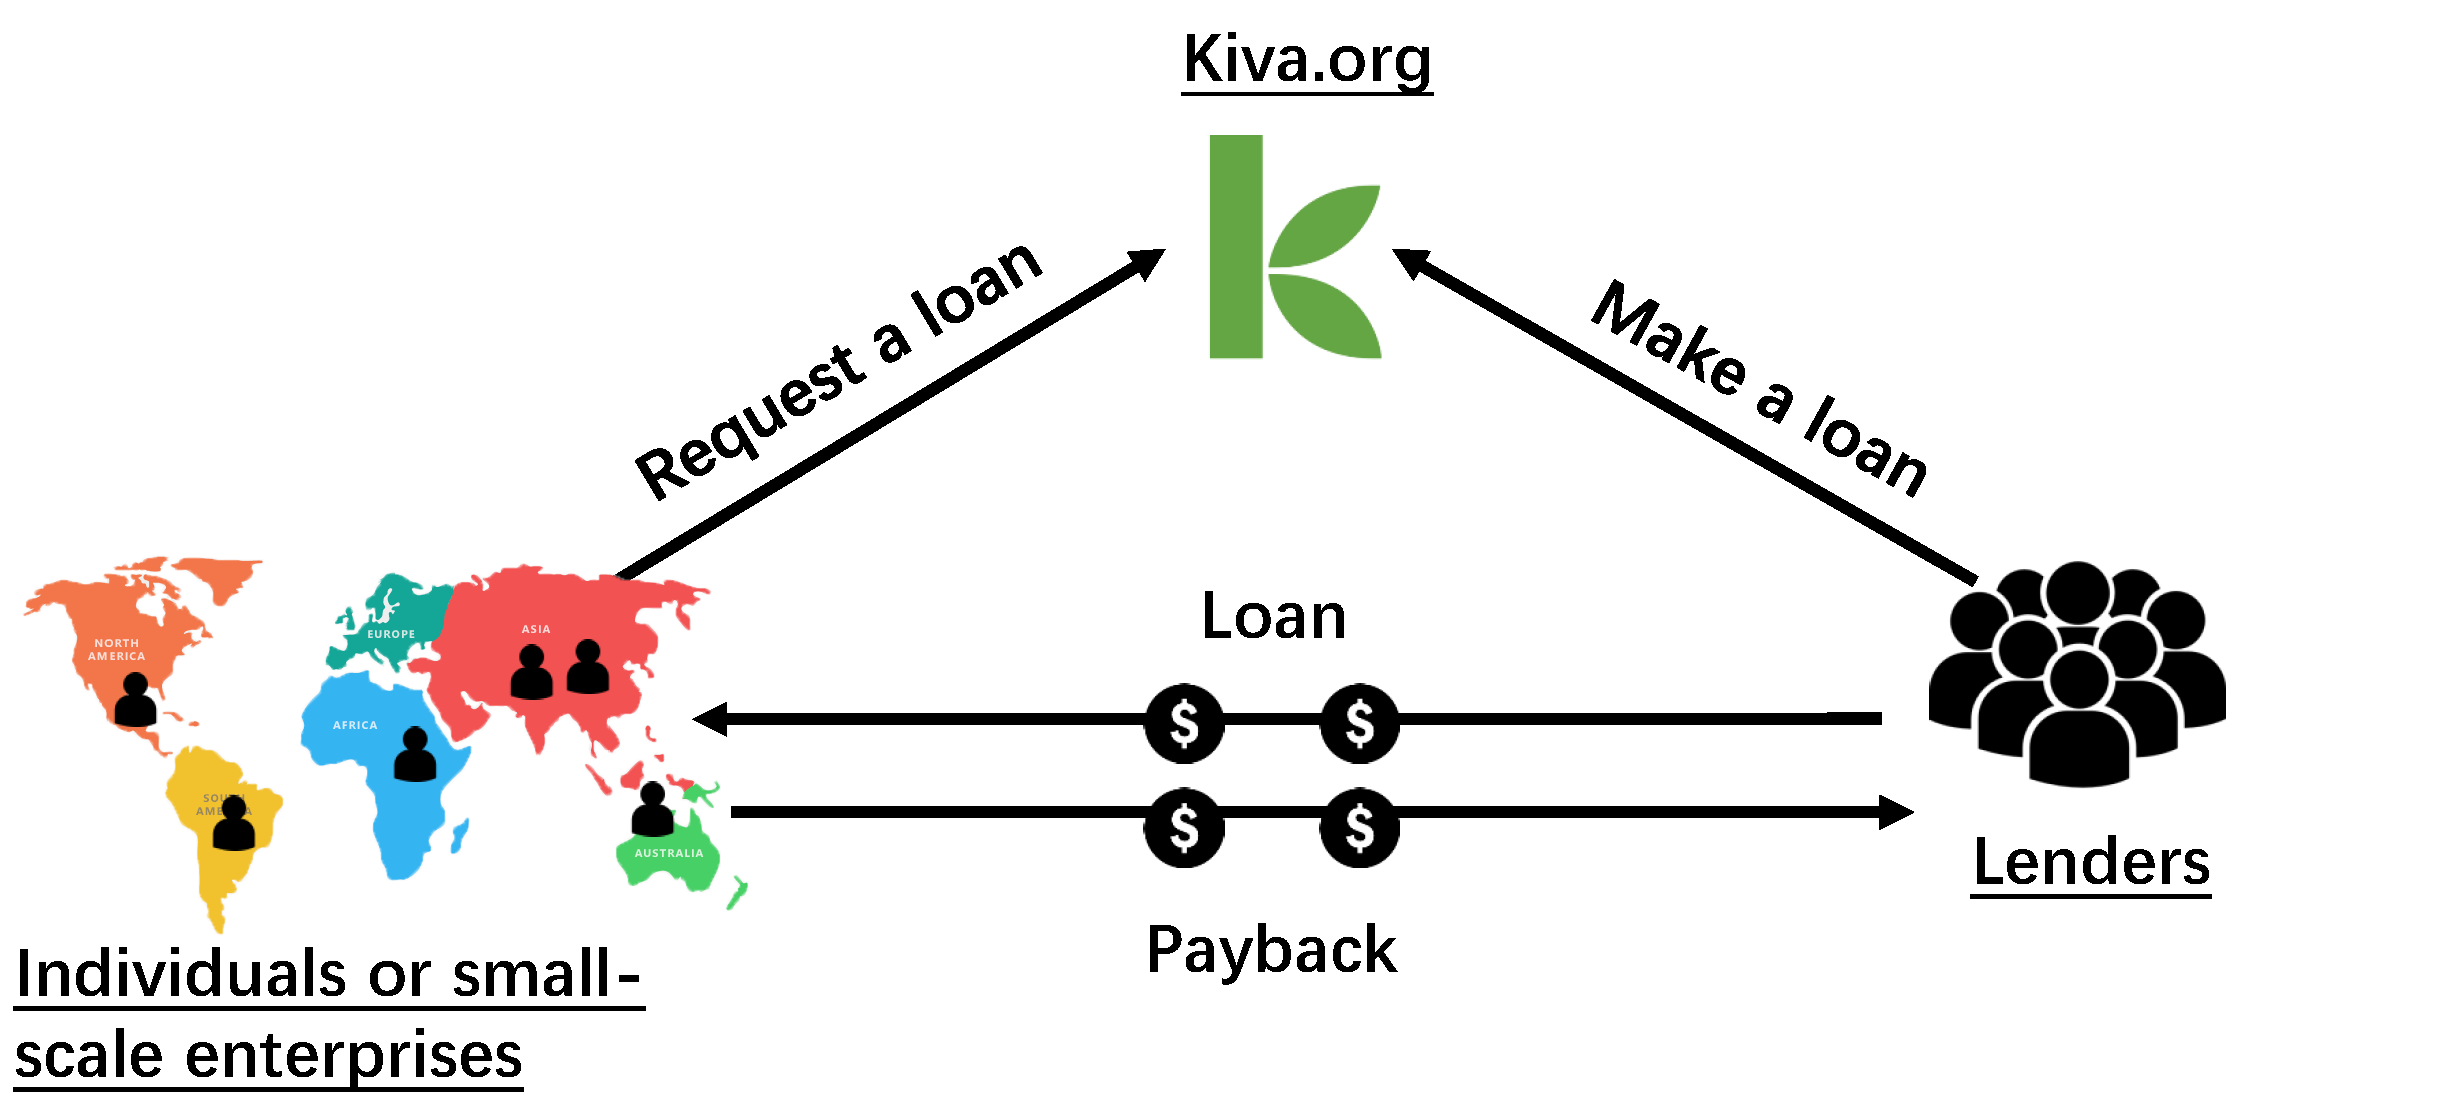
\includegraphics[width=0.98\columnwidth]{imgs/far/microlending.png}
%\vspace{-0.25cm}
\caption{Kiva.org provides an intermediary service for lenders and borrowers.}
\label{fig:kiva_process}
\end{figure}

\begin{figure}
%\vspace{-0.25cm}
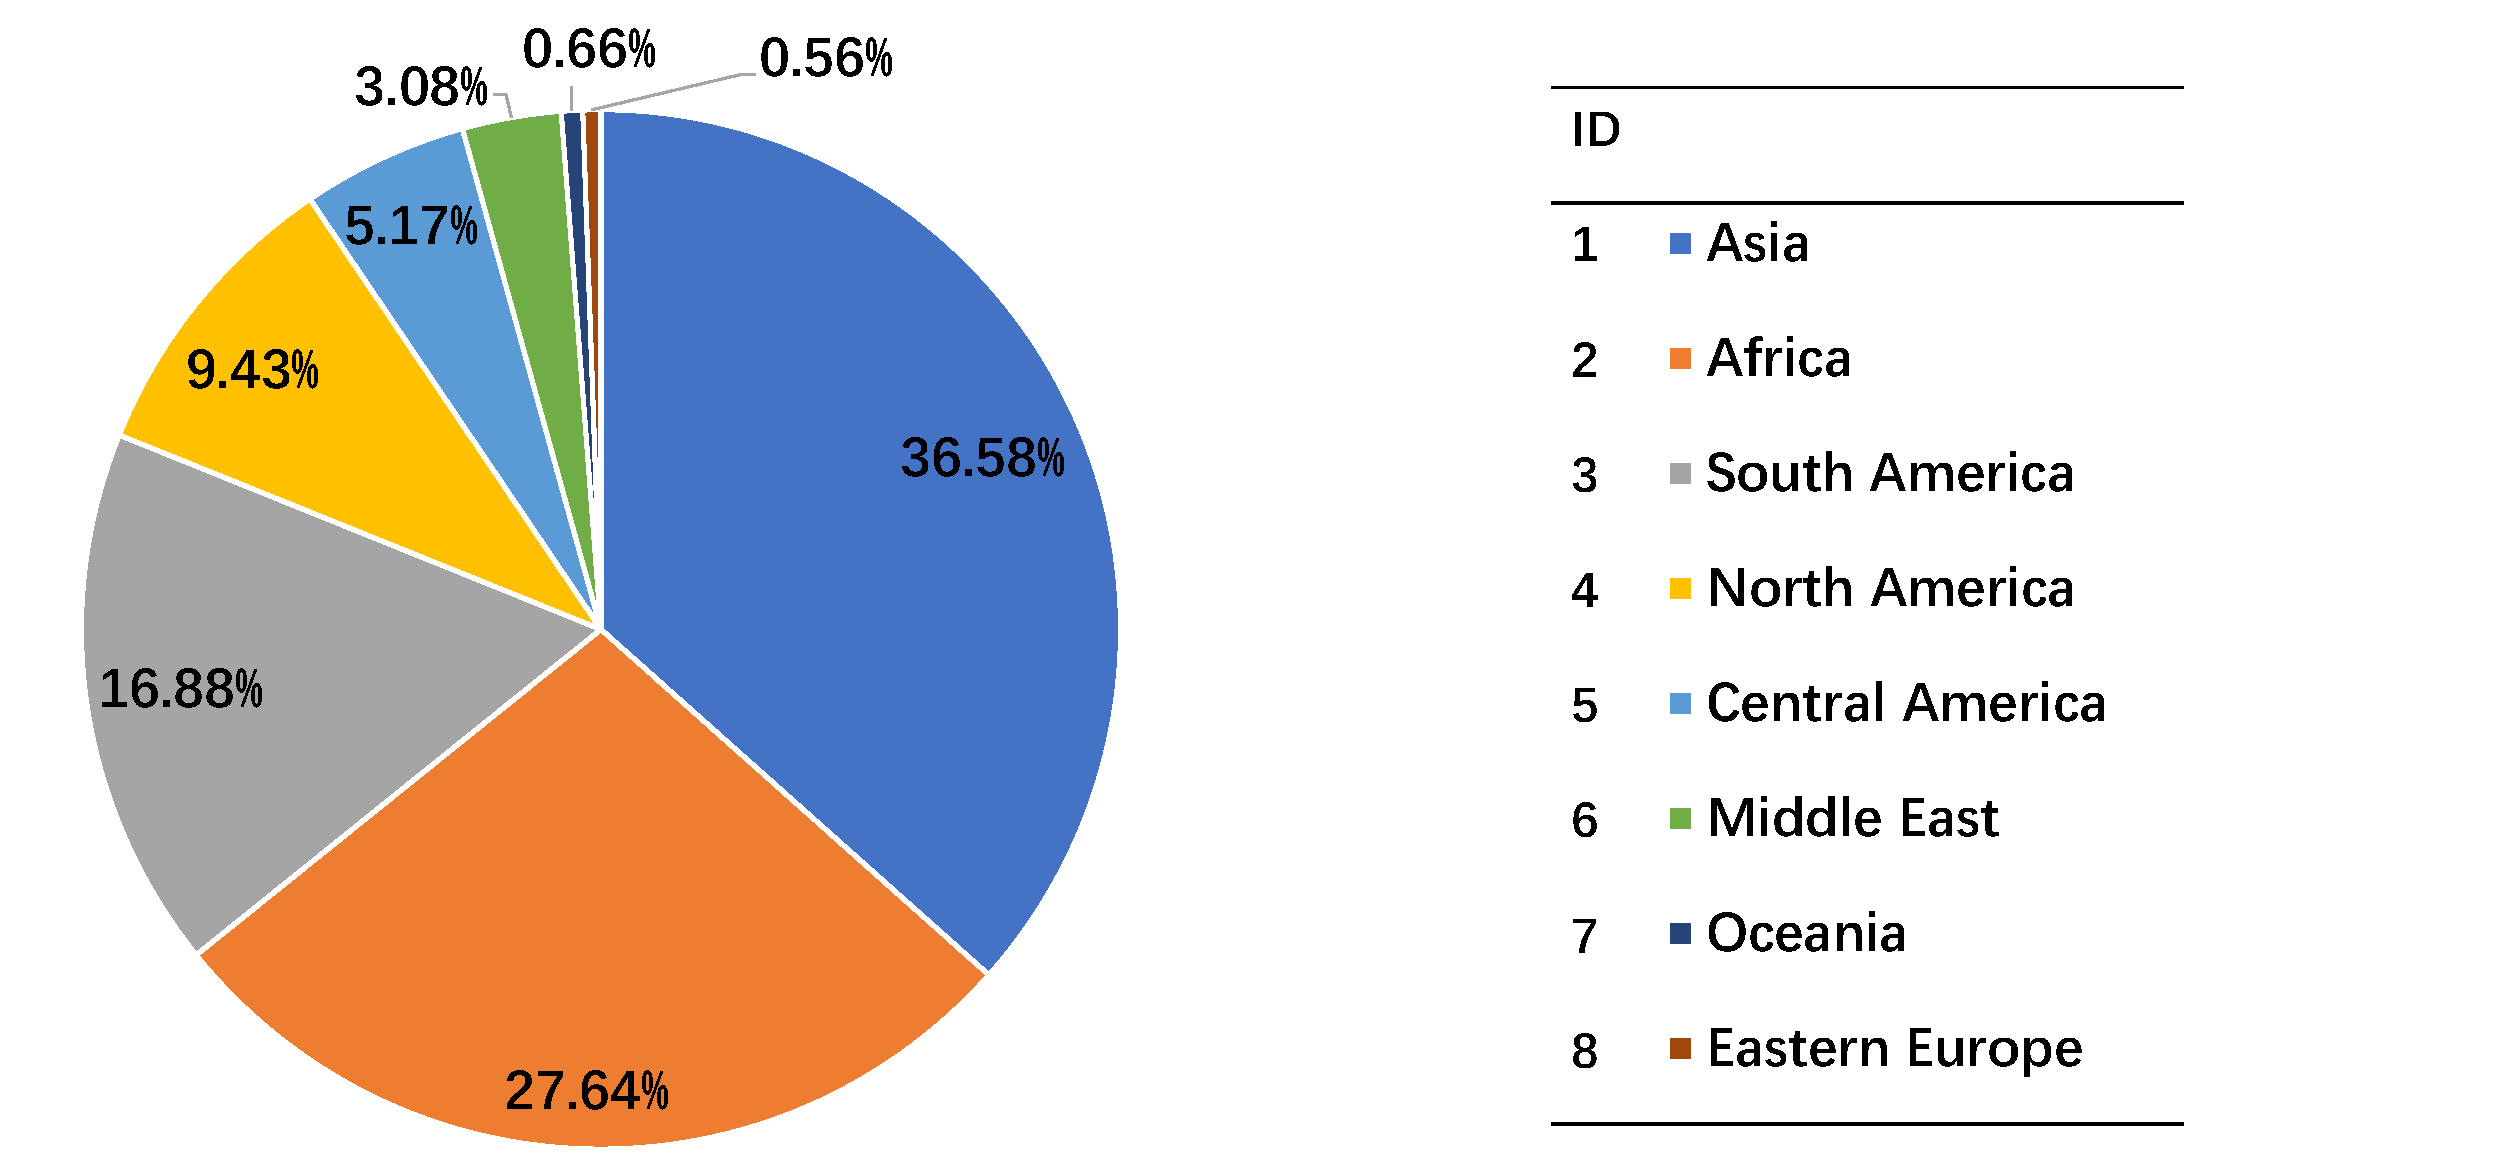
\includegraphics[width=0.98\columnwidth]{imgs/far/kiva.png}
%\vspace{-0.25cm}
\caption{The issue of fairness on regions in a designed loan recommender system \cite{choo2014gather} for Kiva: the recommendation percentage for each region.}
\label{fig:recom_result}
\end{figure}


(i) \textit{Unfair recommendation.} The existing recommender systems for microlending are all lender-centered. These recommender systems have been demonstrated to favor popular items \cite{celma2008hits,lee2014fairness}, resulting in extremely unbalanced recommendation results --- majority groups are usually over-represented, thereby holding a higher proportion of opportunities and resources, while minority groups barely receive exposure. For example, it is observed that certain geographical regions such as Asia and Africa dominate the recommendation in a designed loan recommender system for Kiva~\cite{choo2014gather}; whereas, others like Oceania and Eastern Europe barely receive recommendations, as shown in Figure \ref{fig:recom_result}. Less exposure means the borrowers from these regions are less likely to be funded.

%Moreover, the recommender system will learn the pattern from the historical data that loans from certain regions are less interested, thereby increasing the unfairness.

(ii) \textit{Lender's diversity tolerance.} Another noticeable phenomenon is that lenders' tolerance of diversity varies greatly.  Thus, the diversity of recommended lists should be compatible with the level of each lender's interest in diverse recommendations. For instance, some lenders may highly prefer offering loans to certain regions (such as their home countries), while others may be open to diverse regions. In such scenarios, assuming lenders' diversity tolerance is constant and increasing diversity uniformly for all lenders 
%to improve fairness 
will result in poor recommendations \cite{eskandanian2017clustering}. Therefore, a well-designed recommender system should be personalized by both lenders' interests and the degree of loan diversity in recommended lists.

We aim to design a fairness-aware re-ranking algorithm on top of the existing recommendation algorithms. Our algorithm achieves a balance between recommendation accuracy and borrower-side fairness, and also considers lenders' preferences for diversity. This post-processing step does not depend on any specific recommendation algorithm, and therefore can be widely applied.

% \todo{?}
% \citet{surer2018multistakeholder} suggest a constrained optimization-based method at the post-processing level to enhance fairness for multiple provider groups. This approach is generalizable to multiple constraints, such as a) the inclusion of items from different provider groups, b) ensuring a minimum degree of item diversity for each consumer, and, c) avoiding unfairness towards providers from underrepresented populations.

% \section{The Proposed Algorithm}\label{sect:algorithm}
In this section, we first propose to formulate this recommendation scenario as a Multi-sided Recommender System (MRS) \cite{burke2017multisided, burke2017patterns}.  Then, we design a personalized re-ranking algorithm to achieve a fair recommendation for microlending.

% \begin{figure}
% %\vspace{-0.25cm}
% 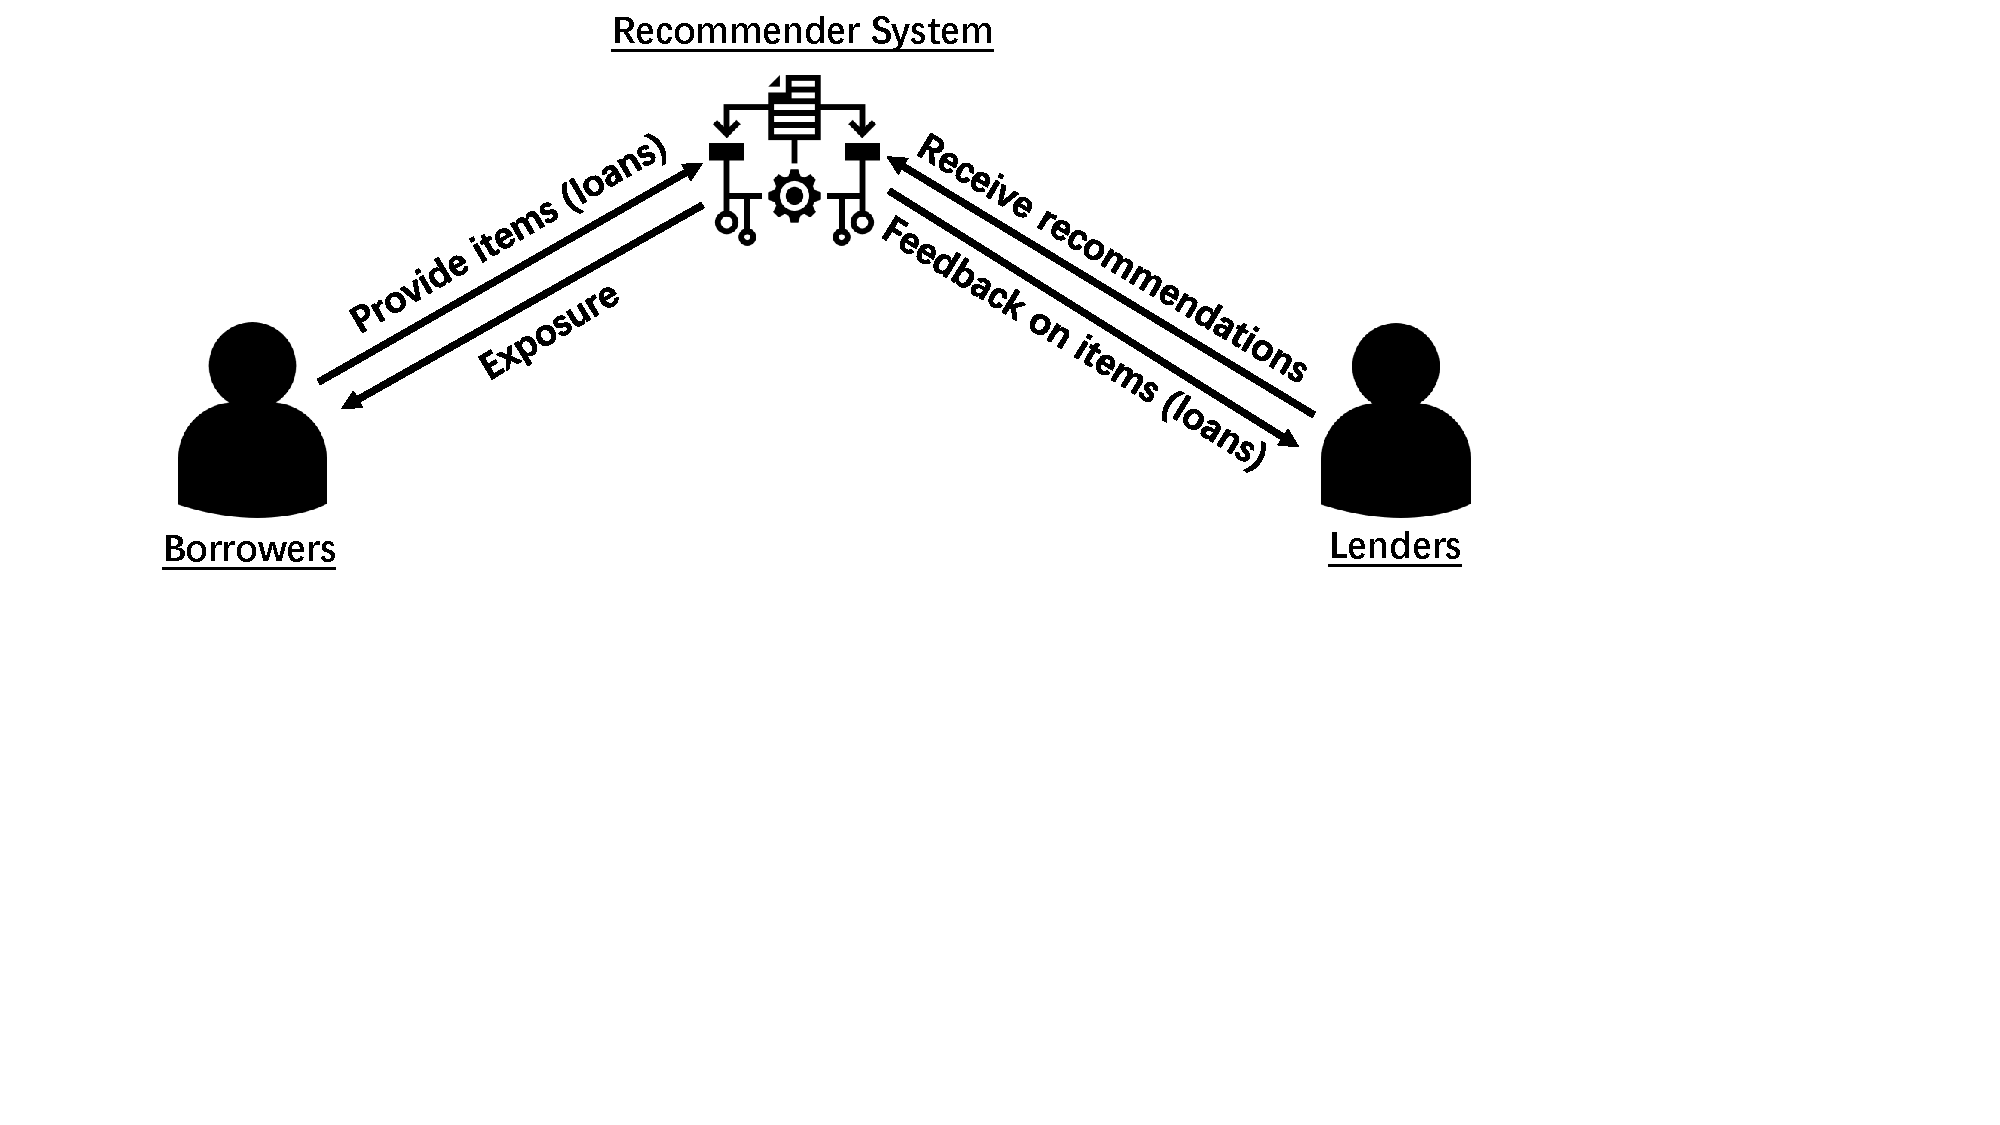
\includegraphics[width=0.99\columnwidth]{imgs/mrs0401.pdf}
% %\vspace{-0.25cm}
% \caption{The recommendation process of a Multi-sided Recommender System (MRS) for Kiva.org.}
% \label{fig:mrs}
% \end{figure}

\subsubsection{\textbf{Problem Formulation}}
\hfill
%Besides maximizing the lenders' interests, we also consider the allocation of recommendation opportunities across the borrower side. 

% The concepts of personalization and fairness are conflicting to some extent \cite{modani2017fairness}. On the one hand, the main goal of personalization is to break the absolute fairness so that the recommended loans can best match the lenders' interests and needs. On the other hand, to obtain the ideal fairness, one could simply divide the recommendation opportunities equally to each region.

% In Kiva.org, different stakeholders are involved, including lenders, borrowers, and the system (Kiva), which can be modeled by an MRS. Borrowers post their loan applications onto the system from which lenders receive loan recommendations. Besides maximizing the lenders' interests, Kiva also aims to consider the allocation of borrower side recommendation opportunities. 

% As we described before, the concepts of personalization and fairness are conflicting to some extent \cite{modani2017fairness}. On the one hand, the main goal of personalization is to break the absolute fairness so that the recommended loans can best match the lenders' interests and needs. On the other hand, to obtain the ideal fairness, one could simply divide the recommendation opportunities equally to each region.


Based on the MRS model, different stakeholders are involved in the loan recommendation setting including lenders, borrowers, and the system (Kiva) where each stakeholder might have a different goal or a different fairness concern. In this system, borrowers post their loan requests on Kiva.org and lenders receive loan recommendations from the system, as depicted in Figure \ref{fig:mrs}. 
Besides maximizing the lenders' interests (personalization), Kiva also aims to consider the allocation of borrower side recommendation opportunities. In other words, Kiva wants to ensure that every loan request (borrower) gets an equal chance of being funded.

% In this paper, we utilize MRS to model the problem of loan recommendation, including lenders, borrowers, and the system. Lenders receive loan recommendations from the recommender system and make loans, as depicted in Figure \ref{fig:mrs}. Borrowers provide items to be recommended to the system by applying for loans. 

% Based on the MRS model, different stakeholders are involved in this recommendation setting including lenders, borrowers, and the system (Kiva), where each stakeholder might have a different goal. In this scenario, Kiva has a fairness objective and wants to ensure that every loan request gets an equal chance of being funded.

To achieve the above goal, given a set of lenders $\mathcal U=\{1,\ldots,n_u\}$, a set of loans $\mathcal V=\{1,\ldots,n_v\}$, and an initial ranking list $R(u)$ for lender $u\in \mathcal U$, our task is to re-rank $R(u)$ and generate a list of $K$ distinct loans $S(u)$ that is both accurate and fair. For a loan $v\in\mathcal V$, $C(v)\in\{1,\ldots,n_c\}$ is the corresponding categorical protected attribute, such as region, race, or gender. Let $\mathcal V_c=\{v|C(v)=c, v\in \mathcal V\}$ denote the \emph{group} of loans with attribute $c$. For instance, if the protected attribute is the geographical region and we use the ID specified in Figure \ref{fig:recom_result}, then $\mathcal V_c$ with $c=1$ represents the set of all loans applied from Asia.


In some contexts, we may separate borrowers into protected and unprotected groups, where the borrowers from the protected group are the particular concern \cite{zliobaite2015survey}. This can be viewed as a special case of our problem with $n_c=2$. In this research, we are looking at more general fairness across all borrower groups and trying to ensure that each re-ranked list $S(u)$ for a specific lender $u$ covers as many borrower groups as possible while considering the personalized constraints for lenders in terms of their willingness to receive a diverse result.
% on diversity tolerance. 
However, we are not allowed to sacrifice too much accuracy to achieve an absolutely fair recommendation result. A tradeoff must be made since accuracy and fairness cannot be fully satisfied at the same time \cite{burke_robin_multisided_nodate}.


\subsubsection{\textbf{Algorithm}}
\hfill

We aim at producing a fairness-aware re-ranking algorithm that can balance personalization and fairness. We assume for a given lender $u$, a ranked recommendation list $R(u)$ has already been generated by a base recommender, \emph{e.g.,} collaborative filtering. The task of our algorithm is to produce a new re-ranked list $S(u)$ containing loans that can satisfy lenders' demands and simultaneously cover as many borrower groups as possible.

We first propose a fairness-aware re-ranking algorithm (FAR) and then incorporate a diversity tolerance term $\tau_u$ to produce the personalized fairness-aware re-ranking algorithm (PFAR).


\paragraph{\textbf{Fairness-aware Re-ranking (FAR)}}
Our proposed Fairness-aware Re-ranking (FAR) criterion is defined as Eq.\eqref{eq:indicator}, which is the combination of a personalization-induced term and a fairness-induced term, with a hyper-parameter $\lambda\in(0,1)$ controlling the tradeoff between the two. For any $u\in \mathcal U$, we solve
\begin{equation}
\max_{v\in R(u)}\;\underbrace{(1-\lambda)P(v|u)}_{\text{personalization}} + \underbrace{\lambda\sum_{c}P(\mathcal V_c)\mathds{1}_{\{v\in \mathcal V_c\}}\prod_{i\in S(u)}\mathds{1}_{\{i\notin \mathcal V_c\}}}_{\text{fairness}},%\; \forall u\in \mathcal U,
\label{eq:indicator}
\end{equation}
where $P(v|u)$ is the personalization score determined by the base recommender, indicating the probability of lender $u$ being interested in loan $v$. The indicator function $\mathds{1}_{A}$ has the value 1 if $A$ is true, and 0 otherwise. The new output list is built iteratively in a greedy manner. At each step, the algorithm selects one loan with the highest re-ranking score from the candidate list $R(u)$ and moves it to the output list~$S(u)$.

%\wwdelete{The re-ranking criterion can be regarded as modelling \textit{personalization} and \textit{fairness}, respectively, with a hyper-parameter $\lambda$ controlling the tradeoff between the two.}
%The personalization score $P(v|u)$ is determined by the base recommender, which is the probability of consumer $u$ being interested in item $v$.

For borrower-side fairness, our idea is to promote the loans that belong to currently uncovered borrower groups. For a loan $v$ that belongs to $\mathcal V_c$, we first compute the coverage of $\mathcal V_c$ for the current generated re-ranked list $S(u)$ as $\prod_{i\in S(u)}\mathds{1}_{\{i\notin \mathcal V_c\}}$, which is equal to 1 if none of the items in $S(u)$ belong to $\mathcal V_c$, and 0 otherwise. If both $\mathds{1}_{\{v\in \mathcal V_c\}}$ and $\prod_{i\in S(u)}\mathds{1}_{\{i\notin \mathcal V_c\}}$ are 1, items that belong to $\mathcal V_c$ are promoted by being assigned a higher score, and thus get a larger chance of being selected. The above process is repeated for each borrower group $\mathcal V_c$, $c={1,\ldots,n_c}$, and the results are summed up. Since each item may belong to multiple groups, the loans belonging to multiple uncovered borrower groups are favored. 

The normalization term $P(\mathcal V_c)$ is determined by the system and indicates the importance of $\mathcal V_c$. For example, if a borrower group is identified as a protected group and receives few recommendations, then the system can assign a higher $P(\mathcal V_c)$ to the corresponding group. For simplicity, we assume a uniform preference over borrower groups and assign an equal $P(\mathcal V_c)$ for all borrower groups.



\begin{algorithm}[t]
\caption{(Personalized) Fairness-Aware Re-ranking (FAR/PFAR)}
\begin{algorithmic}[1]
\REQUIRE $u,R(u),K,\lambda, \tau_u$
\ENSURE $S(u)$
\STATE $S(u)\leftarrow\emptyset$
\WHILE{$|S(u)|< K$}
\STATE Select the optimal $v^*$ by solving $$\arg\max_{v\in R(u)}(1-\lambda)P(v|u)+\lambda\tau_u \sum_{c}P(\mathcal V_c)\mathds{1}_{\{v\in \mathcal V_c\}}\prod_{i\in S(u)}\mathds{1}_{\{i\notin \mathcal V_c\}}$$
\STATE $R(u)\leftarrow R(u)\setminus \{v^*\}$
\STATE $S(u)\leftarrow S(u)\cup\{v^*\}$
\ENDWHILE
\RETURN $S(u)$
\end{algorithmic}
\label{alg:main}
\end{algorithm}

\paragraph{\textbf{Personalized Fairness-aware Re-ranking (PFAR)}}
Note that Eq.\eqref{eq:indicator} is designed for any lender $u\in \mathcal U$. If we simply follow this setting and treat each lender with an equal level of diversity tolerance, then the ranking quality is inevitably suppressed. Actually, lenders' propensity towards diversity varies and different levels of diversity should be considered.

To address this issue, we personalize the previous re-ranking criterion Eq.\eqref{eq:indicator} by adding a personalized weight $\tau_u$ and derive our Personalized Fairness-aware Re-ranking (PFAR) criterion Eq.\eqref{eq:per_indicator}. 
% By incorporating the diversity tolerance, we can further improve the consumer satisfaction and the P-fairness can still be obtained across consumers.
%Built on the previous discussion, we can derive the final form of our Personalized Fairness-aware Re-ranking (PFAR) criterion:
For any $u\in \mathcal U$, we solve

\begin{equation}
\max_{v\in R(u)}\;\underbrace{(1-\lambda)P(v|u)}_{\text{personalization}} + \underbrace{\lambda\tau_u\sum_{c}P(\mathcal V_c)\mathds{1}_{\{v\in \mathcal V_c\}}\prod_{i\in S(u)}\mathds{1}_{\{i\notin \mathcal V_c\}}}_{\text{personalized fairness}},\; %\forall u\in \mathcal U,
\label{eq:per_indicator}
\end{equation}
where the second term considers personalized fairness. The diversity tolerance $\tau_u$ is incorporated to control the weight of the fairness score. If a lender has no special interest to a specific group, the algorithm will focus more on the personalization task. Otherwise, the fairness-induced term can be emphasized.
%is conservative and refuses to see diversified recommendation results, the algorithm will focus more on the personalization task. Otherwise, the fairness-induced term can be emphasized.


To calculate $\tau_u$, we first compute a level of interest $P(\mathcal V_c|u)$ of lender $u$ for each borrower group $\mathcal V_c$, $c=1,\ldots,n_c$,
\begin{equation}
P(\mathcal V_c|u)\buildrel\triangle\over=\frac{\sum_vr(u,v)\mathds{1}_{\{v\in \mathcal V_c\}}}{\sum_{c'}\sum_vr(u,v)\mathds{1}_{\{v\in \mathcal V_{c'}\}}},
\end{equation}
where $r(u,v)$ is the rating from lender $u$ to loan $v$. We compute the ratio of summation over rated borrowers that belong to group $c$ over summation over all the rated borrowers. 

The preference $P(\mathcal V_c|u)\in [0,1]$ indicates the lender's taste over borrower groups where $\sum_{c} P(\mathcal V_c|u)=1$. Some lenders may be highly interested in certain borrower groups, while some lenders may have equal preferences over all the borrower groups. To capture this characteristic, we use the information entropy \cite{shannon2001mathematical} to identify the lender diversity tolerance, namely
\begin{equation}
\tau_u\buildrel\triangle\over=-\sum_{c}P(\mathcal V_c|u)\log P(\mathcal V_c|u),
\end{equation}
where a larger $\tau_u$ means that the lender is more open to a diverse set of borrower groups.

%Note that FAR is a special case of PFAR where $\tau_u = 1$ for any $u\in \mathcal U$. 
The algorithm FAR/PFAR is formally given in Algorithm \ref{alg:main}. For a lender $u$, loans are generated iteratively from the initial ranking list. The loan with the highest score is selected from the candidate list $R(u)$ according to our re-ranking criterion Eq.\eqref{eq:indicator} or Eq.\eqref{eq:per_indicator}. The process is repeated until $S(u)$ has reached the desired length. The proposed algorithm automatically balances personalization and fairness by adding a bonus to the loans that belong to the uncovered borrower groups. The generated re-ranked list for each lender tends to cover each borrower group at least once while encouraging personalization.


\subsubsection{\textbf{Experiments}}\label{sect:exp}
\hfill

In this section, we test our proposed algorithms on a real-world dataset from Kiva.org. The performance of our proposed re-ranking algorithms on top of different base recommenders is evaluated in terms of accuracy and fairness. Our implementation is built upon the LibRec 2.0 \cite{guo2015librec}, and all results are averages from five-fold cross-validation.


\paragraph{\textbf{Dataset}}
Our algorithms are evaluated on a proprietary dataset obtained from Kiva.org, including all lending transactions over an 8-month period. Each loan is specified by features including borrower's name, gender, borrower's country, loan purpose, funded date, posted date, loan amount, loan sector, and geographical coordinates.
%The original Kiva.org dataset has 853,269 transaction records, involving 113,738 different loans and 178,788 consumers (lenders).

One important characteristic of this dataset, and the micro-finance domain in general, is there is rapid turn-over in recommendable items. Loans are only available to lenders for a short period until they are fully funded or dropped from the system. Subsequent visitors will not see or be able to support these loans, limiting the maximum item profile size significantly. For example, at a minimum loan amount of \$25, a \$200 loan can have a maximum of only 8 lenders. Contrasting with a consumer taste domain such as MovieLens \cite{movielens}, where a popular movie might be rated by hundreds or thousands of consumers, the Kiva.org dataset is extremely sparse (with a sparsity of $4.19\times 10^{-5}$) and exhibits a significant item cold-start problem.

To generate a denser dataset with greater potential for user profile overlap, we apply a content-based technique \cite{resnick1997recommender}, creating \textit{pseudo-items} that represent large categories of items. In particular, all loans that share the same borrower gender, borrower country, loan purpose, loan amount (binned to 5 equal-sized buckets), and loan sector are combined into a single pseudo-item. Then we apply a 10-core transformation, selecting pseudo-items with at least 10 lenders who had funded at least 10 pseudo-items. The retained dataset has 11,085 pseudo-items, 9,597 lenders and 204,830 ratings.

\paragraph{\textbf{Comparative Recommenders}}
As of this writing, Kiva.org does not offer recommendation functionality. In our experiments, we assume a context in which the site provides short lists of recommended loans to lenders for their review. We set the protected attribute as the geographical region, because part of Kiva.org's mission is to achieve equitable access to capital across regions. In order to set up the recommendation scenario for Kiva, we select four representative base recommenders to study their performance in accuracy and fairness, as well as how our proposed algorithms can influence the recommendation results: (a) RankSGD \cite{pmlr-v18-jahrer12b} uses stochastic gradient descent to optimize the ranking error; (b) UserKNN \cite{resnick1997recommender}  is a memory-based collaborative algorithm that computes user similarity; (c) Weighted Regularized Matrix Factorization (WRMF) ~\cite{hu2008collaborative} creates a reduced-dimensionality factorization of the rating matrix; (d) Maximum-entropy distribution (Maxent) \cite{choo2014gather} is a loan recommender system specially designed for Kiva. Maxent models lending behaviors by estimating a maximum-entropy distribution based on a set of heterogeneous information regarding micro-financial transactions available at Kiva.


\paragraph{\textbf{Evaluation Metrics}}

We propose to utilize Normalized Discounted Cumulative Gain (nDCG)~\cite{jarvelin2002cumulated} and Average Coverage Rate (ACR) to evaluate recommendation accuracy and borrower-side fairness, respectively. ACR is defined by the average number of borrower groups covered by the ranked list,

% \textit{Normalized Discounted Cumulative Gain (nDCG).}
% Proposed in~\cite{jarvelin2002cumulated}, nDCG is a commonly-used measure of ranking quality, defined as Eq.~\eqref{eq:ndcg}.
% %We follow the convention in recommender systems that there is a gain in DCG (\emph{i.e.,} the item is \textit{relevant}) if the rating of the item in the list is positive.
% \begin{equation}
% \text{nDCG}=\frac{\text{DCG}}{\text{IDCG}},
% \label{eq:ndcg}
% \end{equation}
% where the formula of Discounted Cumulative Gain (DCG) of a $K$ ranked list is defined as
% \begin{equation}
% \text{DCG}=\sum_{i=1}^K\frac{{rel}_i}{\log(i+1)},
% \end{equation}
% where ${rel}_i$ is defined by the ratings of the item in the test set at position $i$. Ideal Discounted Cumulative Gain (IDCG) is the maximum possible DCG, which is the value of DCG computed by sorting all the items in the test set by their ratings.

% \textit{Average Coverage Rate (ACR).}
% To measure the fairness for microlending, we compute the average number of borrower groups covered by the ranked list.
\begin{equation}
    \text{ACR}=\frac{\sum_{u\in U_t}N_{S(u)}}{N_\text{bg}|U_t|},
\end{equation}
where $U_t$ is the test lender set, $|U_t|$ is the number of lenders in the test set, $N_\text{bg}$ is the total number of borrower groups and $N_{S(u)}$ is the number of borrower groups covered in the list $S(u)$. A larger ACR indicates a fairer system regarding borrower-side fairness.

We propose to use Normalized Discounted Cumulative Gain (nDCG) to evaluate the ranking accuracy and borrower-side fairness, respectively.


% \begin{comment}
\textit{Discounted Proportional Fairness (DPF)}
We adopt a well-accepted and axiomatically justified metric of fairness, the proportional fairness \cite{kelly1998rate}. Proportional fairness is a generalized Nash solution for multiple groups.

\begin{equation*}
    DPF=\sum_{i=1}^{n_c}\log\left(\frac{x_c}{\sum_{c'}x_{c'}}\right),
\end{equation*}

where $x_c$ is the allocation utility of group $\mathcal V_c$. We define the utility of $\mathcal V_c$ by the cumulative gain that $\mathcal V_c$ received from all users,
\begin{equation*}
x_c=\sum_{u\in\mathcal U}\sum_{c}\sum_{i=1}^K\frac{{rel}_i\mathds{1}_{\{v\in \mathcal V_{c}\}}}{\log(i+1)}
\end{equation*}
% \end{comment}
Since fairness-aware re-ranking aims to achieve a better tradeoff between fairness and accuracy, we expect that there will be a price to pay for obtaining a fairer system. To study the ACR gain under a certain accuracy budget, we calculate $\text{ACR@NDCG}_{5\%}$, the increased ACR value obtained when we allow a $5\%$ decrease in nDCG. We believe that 5\% nDCG loss may be a reasonable accuracy tradeoff if provider fairness can be enhanced. Indeed, it has been shown that user inconsistency in recommender systems generates a lower bound (the ``magic barrier'') within which accuracy measurements are meaningless, so small relaxations of nDCG may not actually represent a loss in performance~\cite{said2012estimating}.

\paragraph{\textbf{Results and Analysis}}

We first study the performance of applying FAR and PFAR to the base recommenders. We vary the hyper-parameter $\lambda$ from 0 to 1 in steps of 0.1 and record the corresponding ACR and nDCG, where a larger $\lambda$ means the weight of fairness is larger. The results are shown in Figure \ref{fig:kiva_results}. 

\begin{figure}
	\centering
	\begin{subfigure}{0.49\columnwidth} % width of left subfigure
		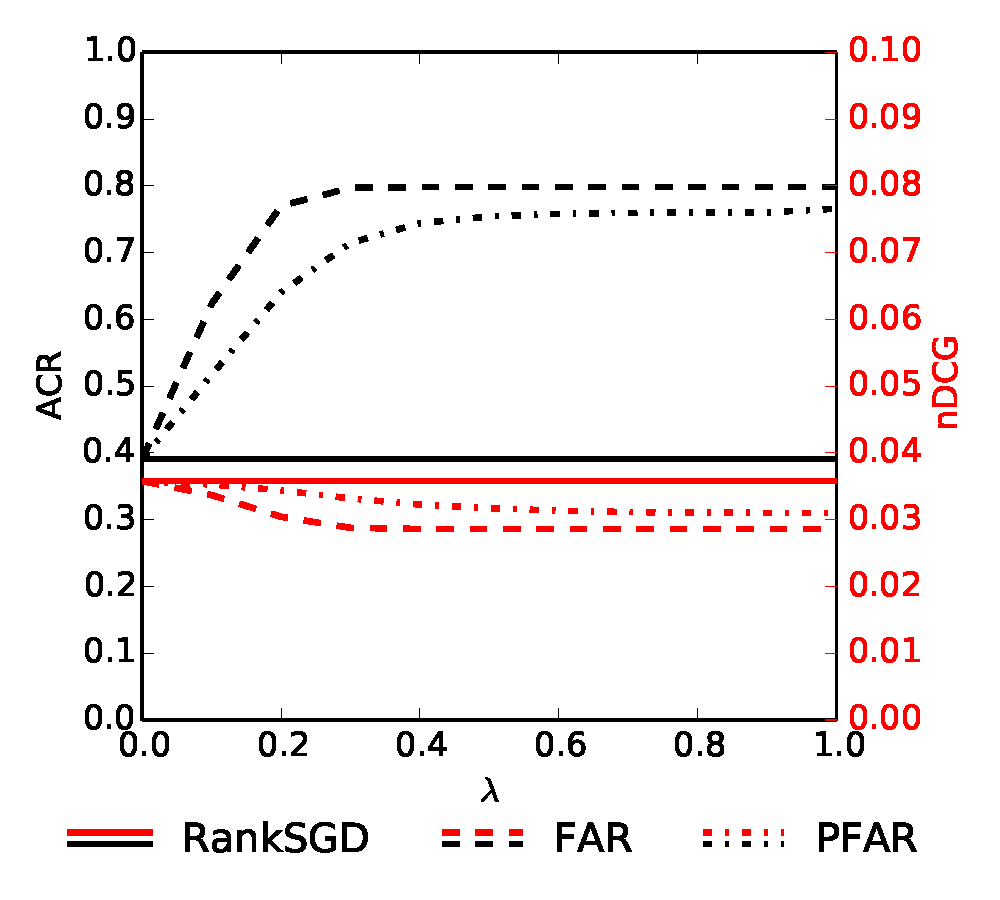
\includegraphics[width=\textwidth]{imgs/far/ranksgd.png}
		\caption{RankSGD \cite{pmlr-v18-jahrer12b}} % subcaption
	\end{subfigure}
	%\vspace{0.2em} % here you can insert horizontal or vertical space
	\begin{subfigure}{0.49\columnwidth} % width of right subfigure
		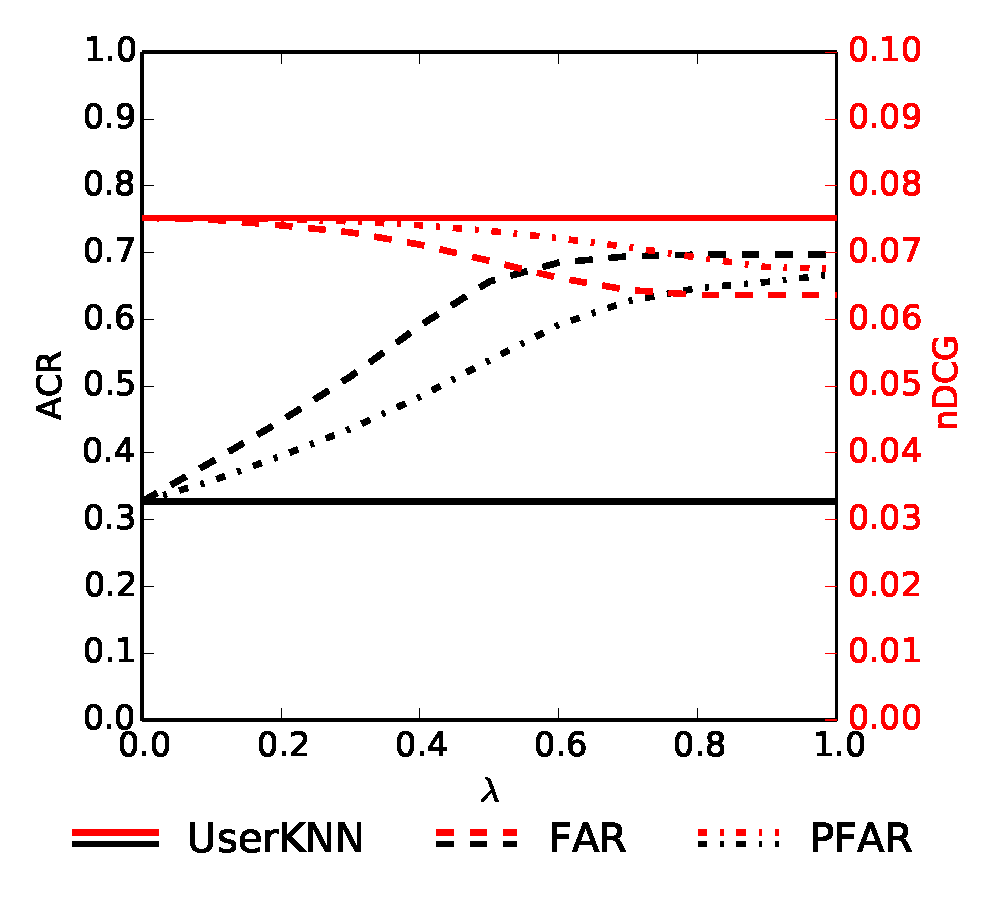
\includegraphics[width=\textwidth]{imgs/far/userknn.png}
		\caption{UserKNN \cite{resnick1997recommender}} % subcaption
	\end{subfigure}
	\begin{subfigure}{0.49\columnwidth} % width of left subfigure
		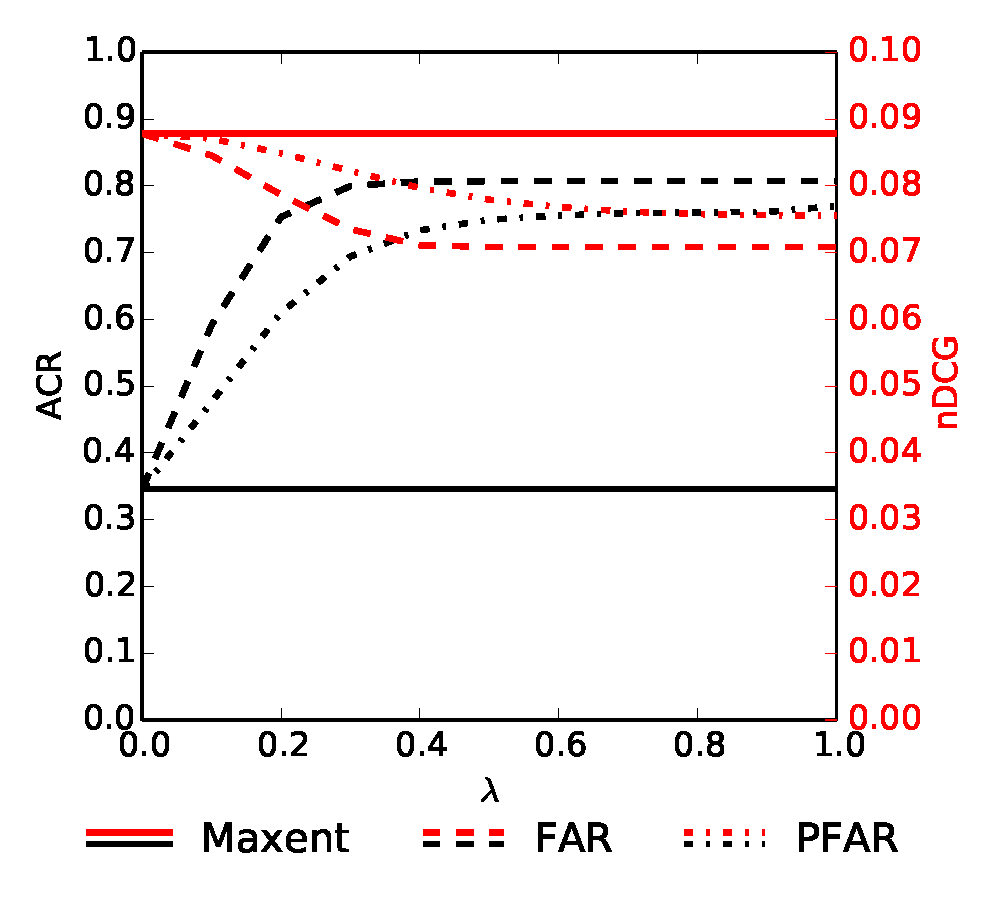
\includegraphics[width=\textwidth]{imgs/far/wrmf.png}
		\caption{WRMF \cite{hu2008collaborative}} % subcaption
	\end{subfigure}
	%\vspace{0.2em} % here you can insert horizontal or vertical space
	\begin{subfigure}{0.49\columnwidth} % width of right subfigure
		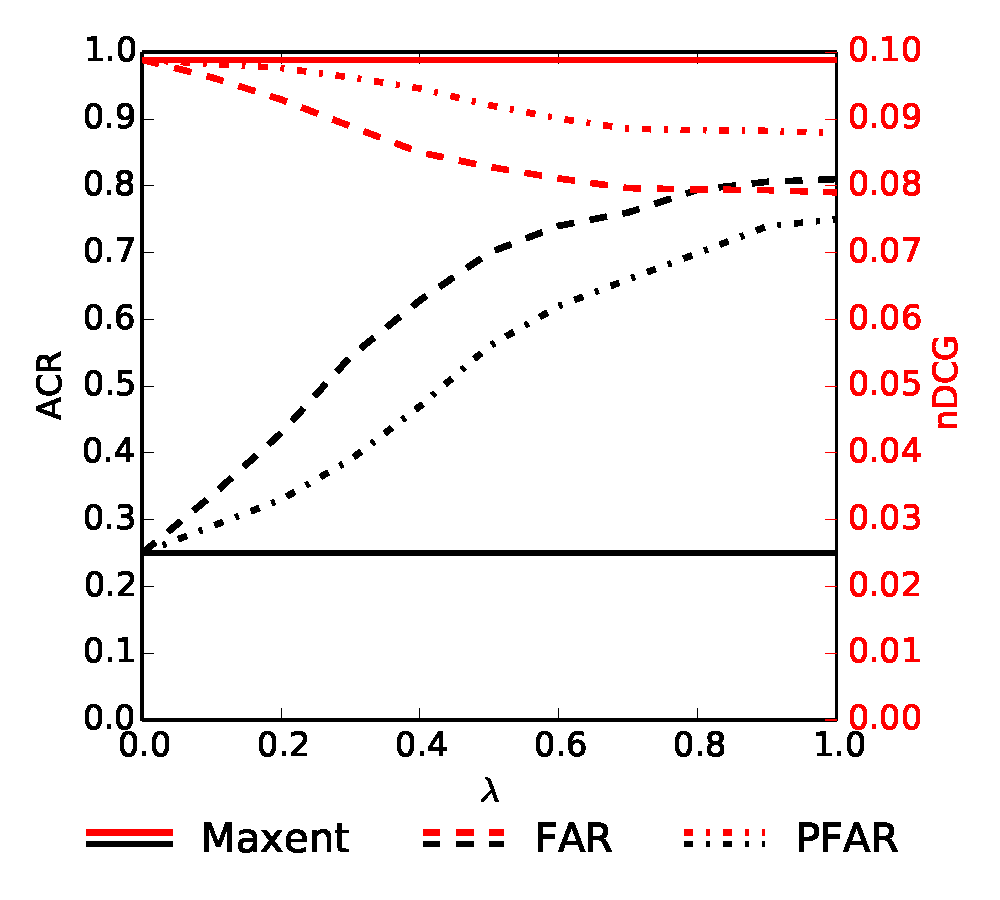
\includegraphics[width=\textwidth]{imgs/far/maxent.png}
		\caption{Maxent \cite{choo2014gather}} % subcaption
	\end{subfigure}
	%\vspace{-0.25cm}
	\caption{Tendencies of ACR and nDCG with increasing $\lambda$.\label{fig:kiva_results}} % caption for whole figure
\end{figure}


Considering the performance of all base recommenders (the solid lines), rankSGD has the lowest accuracy (nDCG = 0.0358); UserKNN comes next with nDCG=0.0752 by finding the nearest neighbors; WRMF performs better than UserKNN by learning the latent factors of lenders and loans (nDCG=0.0878); Maxent obtains the highest nDCG of 0.0988 since Maxent is specially designed for loan recommendation and additional features of loans, \emph{e.g.,} loan sector and geographical coordinates, are utilized. However, accurate recommenders tend to favor items from certain groups, thus resulting in fairness issues.

\paragraph{Effectiveness of the re-ranking algorithms.} By applying our proposed algorithms (when $\lambda\in(0,1)$), all recommenders tend to achieve fairer recommendation results by promoting the loans that belong to less-popular groups, showing the flexibility and effectiveness of our proposed algorithms. Our re-ranking algorithms can be deployed to any base recommender, with the weight of the fairness tunable. The accuracy slightly decreases as $\lambda$ increases, as there is a price to pay for obtaining a fairer system. Take $\lambda=0.1$ for instance, Maxent can obtain a gain of 25.1\% in ACR with a loss of merely 1.6\% in nDCG. Moreover, RankSGD and WRMF converge faster than UserKNN and Maxent with the increase of $\lambda$, indicating that the behavior of our proposed algorithms depends on the initial ranking list to some extent. 

Note that RankSGD has limited ability in learning lenders' preferences, while the results are usually fairer. This is to be expected since accuracy and fairness are conflicting.

\paragraph{Comparison between FAR and PFAR.} The recommendation accuracy of PFAR is higher than FAR, since PFAR limits the amount of loan diversity that the re-ranking imposes, based on the individual tolerance. We can also observe from Figure \ref{fig:kiva_results} that fairness of PFAR is lower, which is consistent with our previous discussion and demonstrates the tradeoff between accuracy and fairness.

%has the highest fairness (ACR = 39.1\%) but the lowest accuracy (nDCG = 0.0358).

% \begin{comment}
% In the first experiment, we plot the tendencies of ACR and nDCG with increasing hyper-parameter $\lambda$, where a larger $\lambda$ means the weight of fairness is larger. Without our proposed re-ranking algorithms (when $\lambda=0$), rankSGD has the highest fairness (ACR = 39.1\%) but the lowest accuracy (nDCG = 0.0358). By utilizing additional content information, \emph{e.g.,} locations of the borrowers, Maxent is the most accurate (nDCG = 0.1) yet unfair (ACR = 25.1\%) recommender. It is because Maxent uses borrower location information as input and learns the biased pattern that lenders are more interested in lending to borrowers from certain regions, which results in an unbalanced recommendation.

% The effectiveness of the proposed re-ranking depends heavily on the quality of the initial ranking list.

% By applying our proposed algorithms (when $\lambda\in(0,1]$), all recommenders tend to achieve fairer recommendation results by promoting the items that belong to less-popular groups. The accuracy slightly decreases as $\lambda$ increases. This is to be expected since accuracy and fairness are conflicting. There is a price to pay for obtaining a fairer system. Interestingly, for Maxent, we could obtain a significant boost in fairness (ACR increases by 71.3\% at $\lambda=0.5$) while accuracy still remains at a high level. The reason may be that Maxent has the ability to discover better items for every borrower group. Therefore, the items may still be attracting for the consumer when promoting the uncovered groups. We also note that the recommendation accuracy is rather low for all base recommenders if we only consider fairness for re-ranking ($\lambda=1$).

% Comparing PFAR to FAR, the recommendation accuracy of PFAR is higher than FAR since PFAR is more personalized and considers the different receptivity of the consumers towards diversified borrower groups. We can also observe from Figure \ref{fig:kiva_results} that the borrower-side fairness of PFAR is lower, which is consistent with our previous discussion and demonstrates the tradeoff between accuracy and fairness.
% \end{comment}



\paragraph{Visualization of the re-ranking results.} We compute the percentage of recommendations for each group with and without the proposed re-ranking algorithms, and study the corresponding allocation distribution. Due to the 4-page limitation, we chose Maxent as an example, and the results are shown in Figure \ref{fig:kiva_num_rec}. Similar trends can be observed for other base recommenders.

(i) The blue bars show the distribution of the base recommender Maxent, \emph{i.e.,} $\lambda=0$. We observe that Maxent focuses on a few major borrower groups, namely Asia and Africa (making up 36.58\% and 27.64\% of total recommendations, respectively), while paying less attention to the others. 

(ii) The ideal fairness is to give each group an equal chance of being recommended. However, accuracy will be significantly downgraded as lenders' preferences are not learned. As a compromise, we find a balance between the two and select $\lambda=0.1$, where the growth rate of ACR per unit nDCG loss is the largest. As illustrated by the green and red bars in Figure \ref{subfig:lambda01}, nDCG still remains at a high level after the re-ranking (nDCG=0.0962 for FAR and nDCG=0.0983 for PFAR), while fairness of the recommendation is significantly improved, as loans belonging to less-popular groups are promoted.

(iii) In Figure \ref{subfig:lambda10}, a larger $\lambda=0.99$ is applied, and the distribution can be even more balanced, while the accuracy is lower.


% To achieve ideal fairness, one would like to give each group an equal chance of being recommended. However, accuracy will be significantly downgraded as lenders' preferences are not learned. As a compromise, we find a balance between the two and achieve a fairer recommendation distribution. We select $\lambda=0.1$, where the rate ACR gain with unit nDCG loss is the largest, and plot the percentage of recommendation of each group of Maxent. Figure \ref{subfig:lambda01} shows that Maxent focuses on a few major borrower groups, namely Asia and Africa (accounting for 36.58\% and 27.64\% of total recommendations respectively), while paying less attention to the others. After the re-ranking, nDCG still remains at a high level (nDCG=0.0962 for FAR and nDCG=0.0988 for PFAR), while fairness of the recommendation is significantly improved, as loans belong to less-popular groups are promoted. In Figure \ref{subfig:lambda10}, a larger $\lambda=0.99$ is applied, the distribution can be even more balanced, while the accuracy is lower.

% Next, we compute the number of recommendations for each provider group, as shown in Figure~\ref{fig:kiva_num_rec}. The weight $\lambda$ is chosen at the maximum unit growth rate of ACR with respect to nDCG. For all base recommenders, the recommendation distribution is unbalanced. Especially for Maxent, almost all recommendations occur in Asia and Africa, accounting for 55.77\% and 34.71\% of total recommendations respectively, while other regions barely get recommended.

% able~\ref{tab:inventory} shows the prevalence of each region in the pseudo-item loan inventory, and demonstrates there is certainly over- and under- representation in the results of all base recommenders. For Oceania, we expect 1/15 loan recommendation as Africa if the recommendation lists were proportional to the inventory. However, Oceania almost has no recommended loans. For PFAR and PFAR, with a reasonable decline in nDCG, regions like Eastern Europe and Oceania are increasingly recommended and the distribution is more balanced.

% demonstrates that the unbalance is not caused by the number of loans each region owns (\emph{i.e.,} the inventory of each region), since the number of recommendations generated by WRMF is not proportional to the inventory.



\begin{figure}
\centering
\begin{subfigure}{0.495\columnwidth}
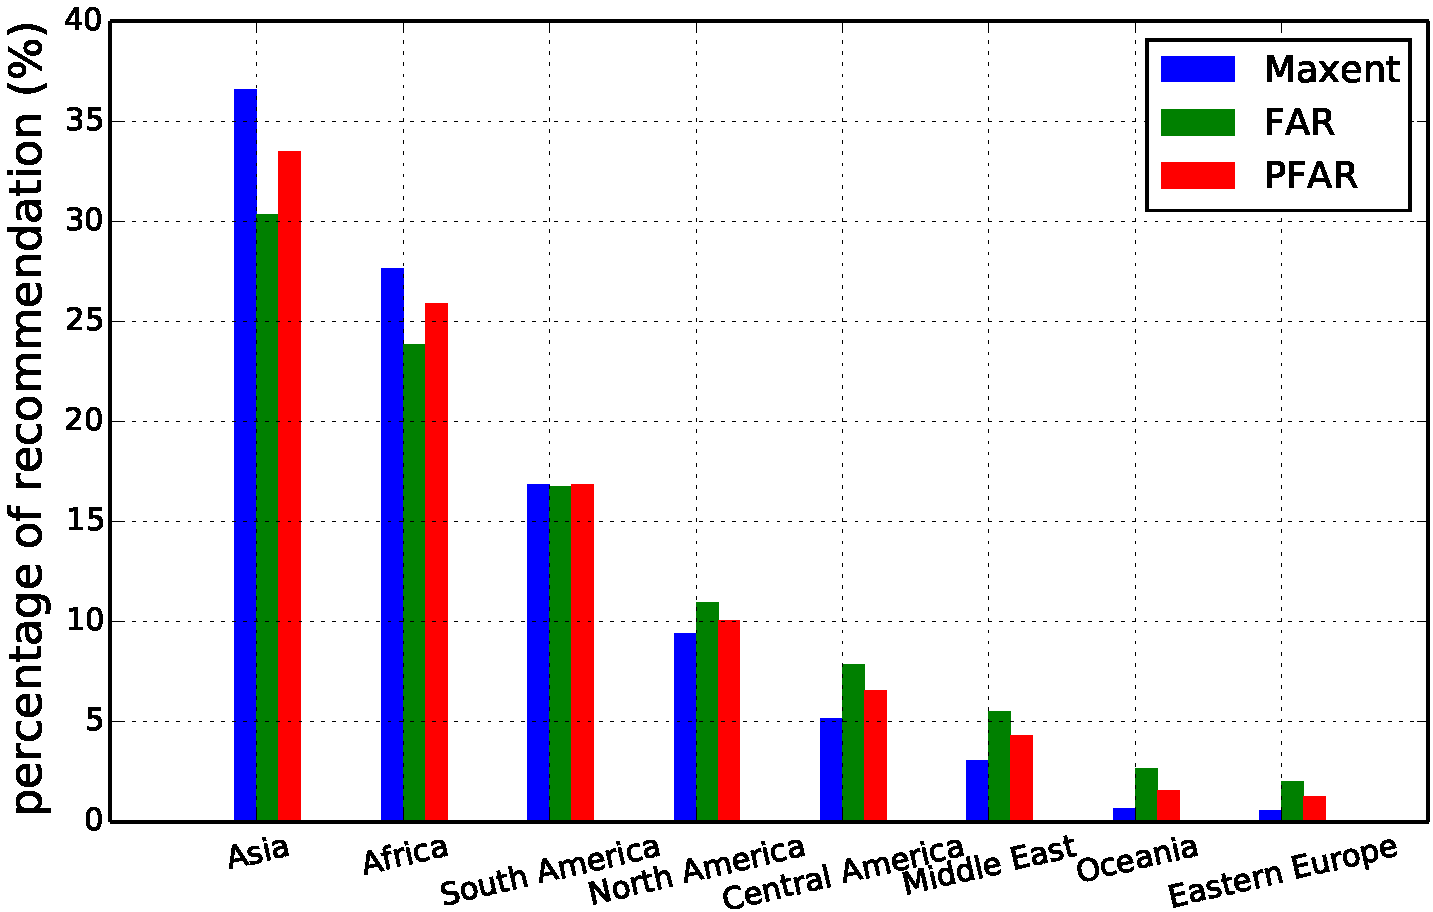
\includegraphics[width=\textwidth]{imgs/far/maxent-lambda01.png}
\caption{$\lambda=0.1$, $\text{nDCG}_{\text{FAR}}=0.0962$,\;\;\;\;\;\; $\text{nDCG}_{\text{PFAR}}=0.0983$. \label{subfig:lambda01}}
\end{subfigure}
\begin{subfigure}{0.495\columnwidth}
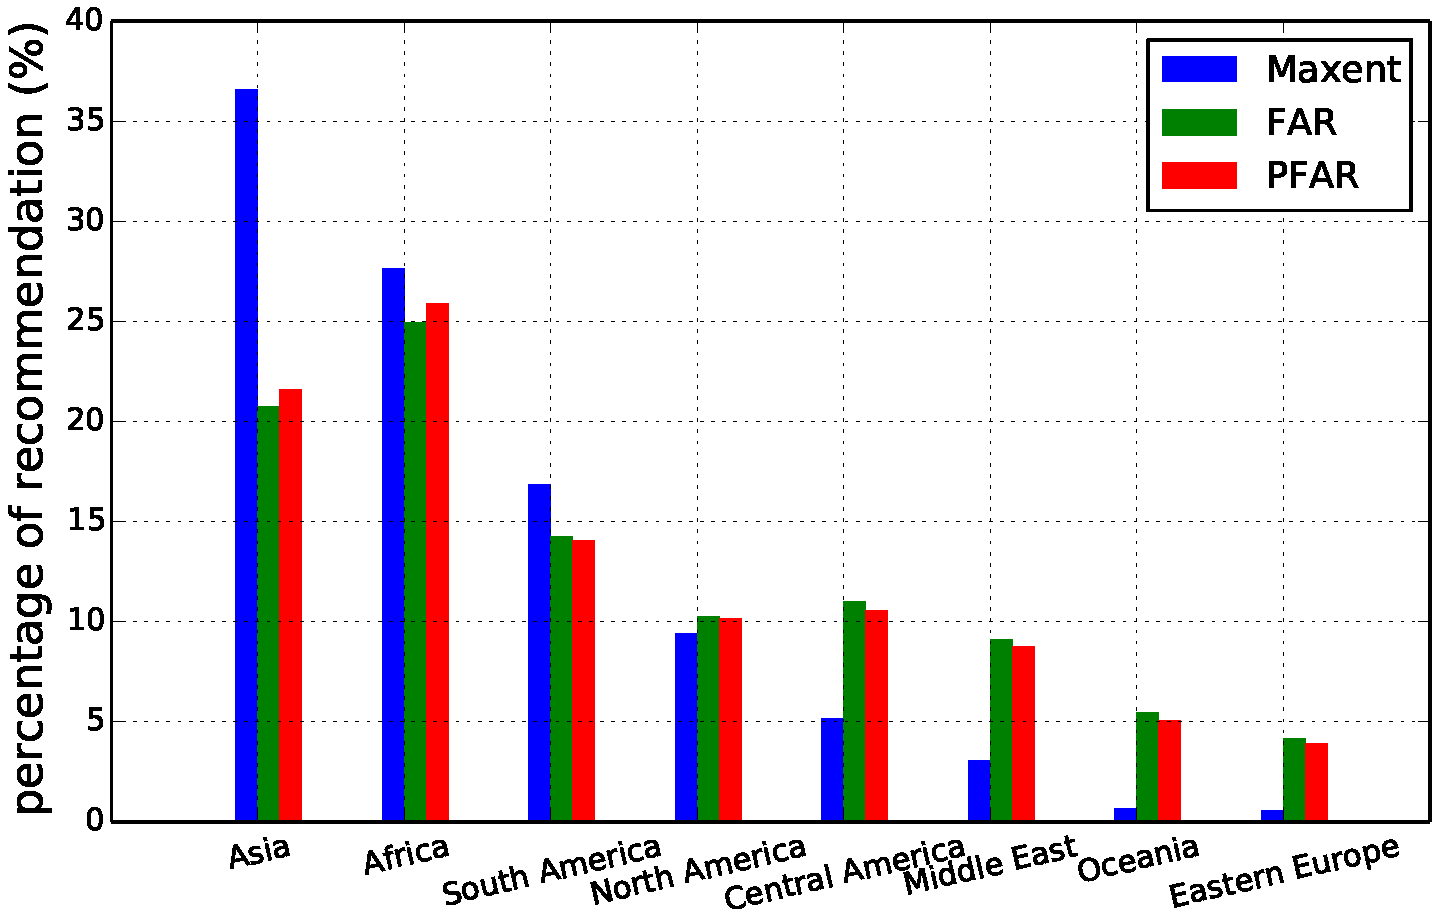
\includegraphics[width=\textwidth]{imgs/far/maxent-lambda10.png}
\caption{$\lambda=0.99$,  $\text{nDCG}_{\text{FAR}}=0.0709$,\;\;\;\;\; $\text{nDCG}_{\text{PFAR}}=0.0756$.\label{subfig:lambda10}}
\end{subfigure}
%\vspace{-0.25cm}
\caption{Recommendation percentage of each region. The blue bars show the results of the base recommender ($\lambda=0$). The green and red bars represent the results of FAR and PFAR, respectively.\label{fig:kiva_num_rec}}
\end{figure}
% The blue bars show the results of the base recommender ($\lambda=0$). The green and red bars represent the results of FAR and PFAR, respectively.


\subsubsection{\textbf{Conclusion and Future Work}}\label{sect:conclusion}
In this work, we proposed a personalized fairness-aware re-ranking algorithm for microlending that can balance accuracy and fairness. We increase the coverage rate of borrowers' regions for Kiva.org to achieve borrower-side fairness, and we show that our algorithm can do so with minimal loss in ranking accuracy. In addition, our algorithm includes lender-specific weights that can be used to personalize the degree of loan diversity.

% In the future, we will consider the position bias into the fairness-aware recommendation for microlending. As discussed in this paper, the recommendation for microlending is moved forward by considering the coverage rate of borrowers and the lenders' diversity tolerance. However, the top positions are generally more valuable than the bottom ones \cite{robertson1977probability}. We plan to make a further assumption that the chance of exposure for an item depends on its position in ranking. Thus, incorporating such position bias into the re-ranking criteria for microlending is promising.

% In the future, we will study a number of variants of our algorithms presented here. We plan to explore different methods for computing personalized diversity tolerance factors, especially to solve the cold-start problem in the current algorithm. We also plan to examine variants of the re-ranking algorithm to take into account the size of each provider group's inventory. 

FAR/PFAR is extremely strict in its requirement that each possible provider group appears at least once at the top of the list. Therefore, another variant to consider is one that can adjust the accuracy/fairness tradeoff in a dynamic way as items are ranked, valuing accuracy more at the top of the list and provider-side fairness more at the bottom of the list.

Finally, we note that, in real-world recommendation applications, managing the tradeoff between accuracy and coverage of provider groups is not a single-shot process. Rather it is an online process, where a current lack of coverage can be compensated for at a later time, and where results are evaluated temporally. This would require making the algorithm sensitive to historical patterns of coverage, rather than just the results obtained in the current list. We intend to explore this type of algorithm design and evaluation in our future work.

This project currently is an on-going project and we intend to develop a method using probabilistic serial allocation and submit it to the ACM Conference Series on Recommender Systems 2021.